\section{Zasada działania}

\subsection{Tor: The Second-Generation Onion Router\protect\footnote{https://svn.torproject.org/svn/projects/design-paper/tor-design.html}}
\begin{description}
  \item Streszczenie
  \begin{description}
   \item Nie wymaga modyfikacji jądra
   \item Nie wymaga specjalnych uprawnień
   \item Zapewnia kompromis pomiędzy zachowaniem anonimowości, użytecznością, oraz wydajnością
   \item Działa "w~prawdziwym Internecie"
  \end{description}

  \item Przegląd (zmiany od generecji 1)
  \begin{description}
   \item Tor to nakładka na sieć, która powstała w~celu anonimizacji aplikacji opartych na protokole TCP (przeglądanie sieci, ssh, wiadomości)
   \item Klient wybiera losowe przekaźniki w~sieci, które przekierowują ruch.
   \item Każdy przekaźnik zna tylko swojego poprzednika, oraz następnika (nie można określić całej ścieżki pakietu, nadawcy i~odbiorcy)
   \item Pakiet jest przesyłany w~komórkach o~stałej wielkości, które są rozpakowywane w~kolejnych węzłach (podobnie jak cebula, stąd trasowanie cebulowe), i~przesyłane dalej
   \item "Perfect forward secrecy"
   \begin{description}
    \item Inicjator negocjuje klucz sesji z~każdym sukcesywnym skokiem w~obwodzie, zamiast przesyłać wielokrotnie zaszyfrowaną wiadomość
    \item Nie potrzebna jest detekcja rejestracji ruchu
    \item Bardziej niezawodne tworzenie obwodów (inicjator wie kiedy skok zawodzi i~może rozszerzyć do nowego węzła
   \end{description}
   \item Separacja "czyszczenia protokołu" od anonimowości
   \begin{description}
    \item Tor używa protokołu SOCKS jako proxy na poziomie aplikacji, który wspiera większość aplikacji opartych na protokole TCP
    \item Opiera się na funkcjach serwerów proxy działających na poziomie aplikacji, pozwalacjących zwiększyć prywatność, takich jak Privoxy\footnote{napisac cos o Privoxy}
   \end{description}
   \item Możliwość udostępnienia wielu strumieni TCP, poprzez jeden zbudowany obwód (nie potrzeba negocjować wielu kluczy publicznych dla każdego połączenia, co daje większą efektywność i~bezpieczeństwo)
   \item Sprawdzanie integralności przesyłanych danych
   \item Punkty spotkania i~ukryte serwisy
  \end{description}
  \item Zasada działania
  \begin{description}
   \item Tor jest nakładką na sieć
   \item Każdy router cebulowy (ang. onion router (OR)) działa jako naromalny proces w~przestrzeni użytkownika, bez żadnych specjalnych uprawnień
   \item Każdy router cebulowy utrzymuje połączenie TLS z~każdym innym routerem cebulowym, z~użyciem kluczy emeferycznych\footnote{Co to są klucze emeferyczne?}
   \item Każdy użytkownik ma uruchomione lokalne oprogramowanie nazywane cebulowym proxy (ang. onion proxy (OP)), które pobiera katalogi, tworzy obwody, oraz utrzymuje połączenia od aplikacji użytkownika
   \item Każdy OR utrzymuje dwa klucze
   \begin{description}
    \item Długoterminowy klucz tożsamościowy
    \begin{description}
     \item Podpisywanie certyfikatów TLS
     \item Podpisywanie opisu routera OR (podsumowanie o~jego kluczach, adresach, przepustowości, polityce wyjścia, itd.)
     \item Podpisywanie katalogów (przez serwery katalogowe
    \end{description}

    \item Krótkoterminowy klucz cebluowy
    \begin{description}
     \item Używany do odszyfrowania zapytać użytkowników, aby skonfigurować obwód i wynegocjować klucze emfiryczne
    \end{description}
    \item Protokół TLS ustanawia krótkoterminowy klucz łącza podczas komunikacji pomiędzy OR.
    \item Krótkoterminowe klucze są okresowo i niezależnie rotowane w celu ograniczenia wpływu na ujawnienie klucza

   \end{description}
   
  \end{description}

\end{description}


\subsection{Komórki}
   \begin{figure}
    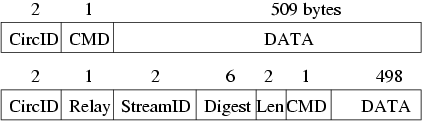
\includegraphics[width=\textwidth]{cell-struct}
    
   \end{figure}

   \begin{description}
    \item Są jednostkami komunikacji w~sieci Tor
    \item Rozmiar komórki: 512 bajtów
    \item Składa się z~nagłówka, oraz treści
    \item Nagłówek
    \begin{description}
     \item CircID (2 bajty) określa do którego obwodu odnosi się komórka (wiele obwodów może być zmultipleksowanych w~jednym połączeniu TLS)
     \item Komenda(1 bajt) opisuje co należy zrobić z~treścią komórki, na podstawie komendy można określić typ komórki:
     \begin{description}
      \item Komórki kontrolne są interpretowane przez węzeł
      \begin{description}
       \item padding - używane do utrzymywania połączeń
       \item create - używane do ustanawiania nowych obwodów
       \item destroy - używane do niszczenia obwodów
      \end{description}

      \item Komórki przekaźnikowe przenoszą dane z~jednego do drugiego końca strumienia
      \begin{description}
       \item Posiadają na początku treści komórki (CircID + CMD + 11 bajtów) dodatkowy nagłówek (nagłówek przekaźnikowy)
       \begin{description}
	\item streamID (2 bajty) - identyfikator strumienia (wiele strumieni może być zmultipleksowanych w~jednym obwodzie)
	\item suma kontrolna (6 bajtów)
	\item długość treści (2 bajty)
	\item komenda "przekaźnikowa" (1 bajt)
	\begin{description}
	 \item relay data - dla danych przesyłanych w~strumieniu
	 \item relay begin - aby otworzyć strumien
	 \item relay end - aby czysto zamknąć strumien
	 \item relay teardown - aby zamknąć uszkodzony strumien
	 \item relay connect(ed) - aby powiadomić OP, że powiodło się rozpoczęcie przekazania
	 \item relay extend(ed) - aby rozszerzyć obwód, oraz do potwierdzania tego
	 \item relay sendme - do kontroli przeciążenia
	 \item relay drop - atrapy dalekiego zasięgu
	\end{description}

       \end{description}
	\item Zawartość nagłówka i~treść komórki przekaźnikowej są szyfrowane i~odszyfrowywane razem w~trakcie przekazywania w~obwodzie, przy użyciu 128-bitowego szyfru AES w~trybie licznika, do wygenerowania "strumienia szyfru?" (ang. cipher stream).
       
      \end{description}

     \end{description}
     
    \end{description}

   \end{description}

\subsection{Obwody i~strumienie}
  \begin{itemize}
   \item Jeden strumien może być współdzielony przez wiele strumieni TCP (podczas połączenia z~witryną internetową tworzonych jest wiele połączeń TCP, co powoduje opóźnienia)
   \item OP okresowo tworzy nowe obwody, jeśli poprzednie zostały użyte, a~te stare już wygasły i~nie mają już żadnych otwartych strumieni.
   \item OP rozważają zbudowanie nowego obwodu co minutę.
   \item Budowanie obwodów odbywa się w~tle (odbudowa uszkodzonego tworzenia obwodu odbywa się bez szkody dla użytkownika)
   
   \item Budowanie obwodu
   \begin{figure}
    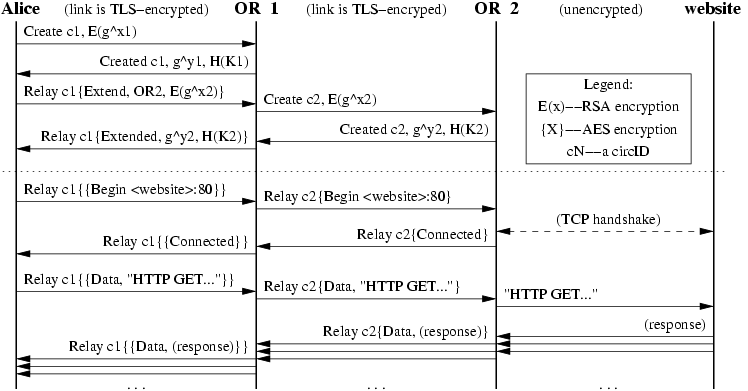
\includegraphics[width=\textwidth]{interaction}
   \end{figure}
   \begin{description}
    \item OP buduje obwód w~sposób przyrostowy (z~każdym skokiem jest negocjowany klucz symetryczny z~każdym OR)
    \item Proces tworzenia obwodu (Alice (OP) --> Bob (OR1) --> Carol (OR2) --> ...)
    \begin{enumerate}
     \item (A -> B) Alice wysyła komórkę typu \textit{create} do pierwszego węzła (Boba)
     \begin{itemize}
      \item Alice wybrała nieużywany w~połączeniu od niej do Boba circID $C_{AB}$ 
      \item Treść (payload) komórki zawiera pierwszą połowę procesu uzgadniania klucza za pomocą protokołu Diffiego-Hellmana $g^x$, zaszyfrowaną do klucza cebulowego (publicznego) Boba
     \end{itemize}
     \item (B -> A) Bob odsyła odpowiedź Alice w~komórce typu \textit{created}, zawierającej drugą połowę procesu uzgadniania klucza $g^y$, wraz z~hashem wynegocjowanego klucza $K=g^{xy}$
     \item Obwód zostaje ustanowiony
     \item Alice i~Bob mogą wysyłać do siebie komórki typu \textit{relay extended}, zaszyfrowane za pomocą wynegocjowanego klucza (obecnie klucz ten jest używany do dzielenia się dwoma kluczami symetrycznymi, dla każdego kierunku komunikacji)
     \item (A -> B) Alice wysyła komórkę typu \textit{realy} do Boba. 
     \begin{itemize}
      \item Określany jest adres następnego węzła (Carol)
      \item Wysyłana jest pierwsza część zaszyfrowanego procesu uzgadniania klucza DH $g^{x_2}$
     \end{itemize}
     \item (B -> C) Bob kopiuje $g^{x_2}$ do komórki typu \textit{create} i~wysyła ją do Carol w~celu rozszerzenia obwodu
     \begin{itemize}
      \item Bob wybiera nowy, nieużywany do połączenia pomiędzy nim a~Carol circID $C_{BC}$
      \item Bob powiązuje $C_{AB}$ z~$C_{BC}$
     \end{itemize}
     \item (C -> B) Carol opowiada komórką typu \textit{created}
     \item (B -> A) Bob pakuje treść (payload) komórki w~komórkę typu \textit{relay extended} i~wysyła ją z~powrotem do Alice
     \item Obwód jest rozszerzony o~węzeł Carol. Alice i~Carol współdzielą wspólny klucz $K_2=g^{x_2y_2}$
     \item W~celu rozszerzenia obwodu, Alice powtarza powyższy proces zawsze wysyłając wiadomość do ostatniego węzła w~obwodzie

    \end{enumerate}
    \item Protokół realizuje jednostronne uwierzytelnianie (OR nie wie kto otwiera obwód, Alice nie używa klucza publiczego i~pozostaje anonimowa)
   \end{description}

  \end{itemize}
  
  \subsection{Sprawdzanie integralności w~struminiach}
  \begin{description}
    \item W~poprzedniej wersji Trasowania Cebulowego nie była sprawdzana integralność plików, co sprawiało, że osoba atakująca mogła zmienić typ komórki na \textit{destroy}, zmienić adres przeznaczenia na swój serwer, lub zmienić komende FTP na np. rm *
    \item Integralność jest sprawdzana tylko na krawędziach strumienia (krawędzią strumienia może być każdy skok w~obwodzie)
    \item Kiedy Alice negocjuje klucz z~każdym nowym skokiem, każdy z~nich inicjalizuje skrót SHA-1 z~pochodną tego klucza (ang. SHA-1 digest with a~derivative of that key), rozpoczynając od losowych wartości, które są znane tylko przez dwóch z~nich
    \item Każdy z~nich dodaje przyrostowo do skrótu SHA-1 zawartości wszystkich komórek typu \textit{relay}, które stworzyli i~dołączają z każdą komórką \textit{relay} pierwsze 4 bajty obecnego skrótu (w~celu zmniejszenia narzutu)
    \item Poza tym każdy zachowuje skrót SHA-1 otrzymanych danych, aby zweryfikować, czy otrzymane hashe są prawidłowe 
    \item Jeśli OP lub OR otrzyma zły hash, to obwód zostaje zniszczony (ang. tear down)
  \end{description}

\subsection{Ograniczenia oceny?? i uczciwości}
\begin{description}
  \item 
\end{description}
   
\begin{description}
 \item Ogólna zasada działania + odnośniki do obrazków
 \item Używane protokoły
 \begin{description}
  \item Warstwy transportowej (TCP, czy UDP)
  \item Warstwy aplikacji (SOCKS)
  \item 
 \end{description}
 \item serwery filtrujące (Privoxy)
 \item serwery pośredniczące
 \item algorytm szyfrujący
 \item długość kluczy szyfrujących
 \item obrazki ilustrujące zasadę działania
\end{description}

\subsection{Ukryte serwisy}
\begin{description}
 \item Nie potrzeba używać firewalla
 \item Specjalna pseudodomena .onion
 \item Losowo wygenerowane adresy serwisów
\end{description}

\subsection{Użycie sieci Tor na systemie Linux i/lub Windows}
\begin{description}
 \item Kolejne kroki + output z terminala
 \item Dowód działania
\end{description}

\subsection{Utworzenie ukrytego serwisu w systemie Linux}
\begin{description}
 \item Kolejne kroki + output z terminala
 \item Dowód działania
\end{description}

\subsection{Przyłączenie się do serwerów pośredniczących}
\begin{description}
 \item Kolejne kroki + output z terminala
 \item Dowód działania
\end{description}

\subsection{Trasowanie Cebulowe}
